\documentclass[11pt]{article}
\usepackage{amsmath,amssymb,amsthm,enumerate,graphicx,hyperref,tikz}
\usetikzlibrary{arrows.meta}

\newtheorem{theorem}{Theorem}
\newtheorem{lemma}[theorem]{Lemma}
\newtheorem{definition}[theorem]{Definition}
\newtheorem{proposition}[theorem]{Proposition}
\newtheorem{corollary}[theorem]{Corollary}
\newtheorem{example}[theorem]{Example}

\title{Horn Retraction, Roth Extremals, and Espresso-Horn\\
for Certified Cyclic-Core Covering}
\author{Alan J.\ Coppola\thanks{Optn gn Software. \texttt{ajjc@optngn.com}} \and
Bala Krishnamoorthy\thanks{Washington State University. \textit{(proposed co-author)}}}
\date{arXiv Wave~1 freeze 2026-11-24}

\begin{document}
\maketitle

\begin{abstract}
We treat the cyclic core of two-level logic minimization as a \emph{cubical
complex} in the sense of Quine--McCluskey and Roth~\cite{roth1957}: primes are
elementary cocycles, essentials are $0$-dimensional $L$-extremals, and
codimension-$1$ free faces survive in over $95\%$ of nontrivial $n=5$ cores.
Classical Espresso-family heuristics (\textsf{REDUCE}/\texttt{sccc}, Signature,
BOOM, ABC ISOP) and exact solvers stop topological reduction when essentials
vanish.  We elevate \emph{Horn retraction}
$\Lambda_f(f_{\mathrm{top}})=\partial f_{\mathrm{top}}\setminus\{f\}$
(Theorems~H1--H4) as the main exact / bounded-approximate / probabilistic
extension: it preserves residual coverage and $H^*(K;\mathbb{F}_2)$, escapes
\texttt{sccc}-locked local minima (Theorem~E1), and tightens the certified
window $L=\max(L_{\mathrm{MIS}},\lceil z_{\mathrm{LP}}\rceil)\le\mathrm{opt}\le U$.
\textsf{TopoSpine}'s non-vacuous \textsf{HornRetractionCollapsePass} reduces the
2007 core where single-face covering collapse stalls; Lean~4 certifies the
Roth/Espresso-Horn lemmas with zero \texttt{sorry}.  Two-dimensional grid
surrogates are deferred to the companion note \texttt{intuition\_examples.pdf}.
The program-level TDA companion is Paper~E~\cite{paperE}.
\end{abstract}

\noindent\textbf{Keywords:} logic minimization, cubical complexes, Horn retraction,
cyclic core, Espresso, certified covering, Lean~4.

\section{Introduction}
\label{sec:intro}

Minimum-cost unate covering is the computational kernel of two-level Boolean
minimization~\cite{quine1952,mccluskey1956,coudert1994}.  Branch-and-bound on
the covering table iterates essentials, row/column dominance, and partitioning
until a fixed point---the \emph{cyclic core}---where classical exact solvers
(Espresso-EXACT, Scherzo) and Espresso-II~\cite{brayton1984} typically branch
two-way or enter \textsf{REDUCE}/\texttt{sccc} local search~\cite{goldberg2000}.
Espresso-Signature~\cite{mcgeer1993}, BOOM coverage-directed
search~\cite{fiser2003}, ABC's Minato--Morreale ZDD ISOP, and LP/ILP bounds
(HiGHS) provide complementary baselines.

Following Roth~\cite{roth1957} and Coppola~\cite{coppola1989,coppola2007}, we
represent primes as cubes in a \emph{cubical complex} $C(f)$.  Roth's
$0$-dimensional extremals are essentials; we treat free faces as
\emph{higher-dimensional Roth extremals}.  Whitehead's elementary collapse
removes $R_f=\{f,f_{\mathrm{top}}\}$ and retracts onto the
\emph{horn}~$\Lambda_f(f_{\mathrm{top}})$, strictly dominating single-face swap
and enabling controlled collapsible chains compatible with Forman / modern TDA
persistence pipelines.

\paragraph{Contributions.}
\begin{enumerate}
\item Layer~0 cube-array definitions: legal expansions, cyclic cores, free faces,
and zero-loss Roth push-down (Section~\ref{sec:defs}--\ref{sec:layer0-main}).
\item Constructive Theorems~H1--H4 and Theorem~E1: Horn retraction, cylinder /
cone-prism, complement-boundary duality, controlled horn chains in exact /
bounded-approx / probabilistic modes, and Horn escape from Espresso
\textsf{REDUCE} stalls with LP/MIS tightening (Section~\ref{sec:horn-chains}).
\item \textsf{Espresso-Horn} and head-to-head variants
(\textsf{espresso\_ii}, Signature, BOOM CD-Search, ABC ISOP, HiGHS LP/ILP) plus
a non-vacuous \textsf{HornRetractionCollapsePass} in \textsf{TopoSpine}
(Section~\ref{sec:experiments}).
\item Lean~4 modules \textsf{HornChains} / \textsf{RothEspressoHorn} (zero
\texttt{sorry}); Layer~1 grid intuition isolated in
\texttt{intuition\_examples.pdf}.
\end{enumerate}

\section{Definitions}
\label{sec:defs}

\noindent\textit{Layer~0 (home problem).}  Absolute minimization starts from an
\emph{array of cubes} covering an ON-set of minterms (minterms may be implicit).
Canonical glossary: \texttt{docs/definitions-cube-array.md}.

\begin{definition}[Array of cubes, legal expansions, and absolute minimum]
\label{def:array-cubes}
Let $C=\{c_1,\ldots,c_k\}\subseteq\{0,1,-\}^n$ be an input \emph{array of cubes}
implicitly defining the ON-set $F=\bigcup_{i=1}^k\mathrm{minterms}(c_i)$.  For the
\emph{absolute minimization} problem, candidates are not restricted to subsets of
$C$: \emph{legal expansions} (single-cube literal raising checked by cube
containment $c'\subseteq\bigcup C$, absorption, and consensus $a*b$) expand cubes
toward the prime implicants $P(F)$ without enumerating $2^n$ minterms.  The
\emph{absolute minimum} is
$\mathrm{opt}(F)=\min\{|S|:S\subseteq P(F),\ S\text{ covers }F\}$.
\end{definition}

\begin{definition}[Cubical complex $C(f)$]
Let $f:\{0,1\}^n\to\{0,1\}$ with ON-set $F$.  Let $P$ be the set of prime
implicants (maximal cubes in $F$).  The \emph{prime cubical complex}
$C(f)=(\mathrm{Skel},\le,\dim)$ is the closure of $P$ under intersection and
face relations (see~\cite{coppola2007}).
\end{definition}

\begin{definition}[Covering table (Layer~0)]
\label{def:covering-table}
Rows are taken from the cover domain (classically ON-set minterms; graded tables
may use product terms and faces); columns are cubes $p\in P$.  Entries
$\mathrm{Pair}(c,p)=1$ iff $c\le p$ (containment / face relation).  Minterms need
not be listed explicitly when containment is determined by the cubes.  When a row
is jointly coverable but not containable in any single prime, lazy cofactor
splitting restores correctness (Lemma~\ref{lem:refine}).
\end{definition}

\begin{lemma}[Lazy row refinement]
\label{lem:refine}
Splitting a row cube $c$ into cofactors $c|_{x=0}$ and $c|_{x=1}$ along a
free coordinate preserves the minimum-cost cover value: a prime set covers
$c$ iff it covers both cofactors.
\end{lemma}

\begin{definition}[Cyclic core]
\label{def:cyclic-core}
The \emph{cyclic core} is the residual covering problem after legal expansions
and legal reductions (essential-prime extraction via cube difference
$p\setminus\bigcup_{q\ne p}q\ne\emptyset$ or unique-row essentials, row/column
dominance, zero-loss free-face push-down, and connected-component
\emph{blob} partitioning) reach a fixed point.  By definition it has no essential
primes and no dominated rows/columns.
\end{definition}

\begin{definition}[Collapsible cube]
A cell $c$ in a cyclic core is \emph{collapsible} if it has a face $f<c$ with
$\dim f=\dim c-1$ that is not a face of any other remaining cell
(a \emph{free face}).
\end{definition}

\begin{definition}[Collapse-branch]
Given collapsible column (prime) $p$ with free faces $F(p)$: remove $p$, add
columns for cubes in $F(p)$, recurse once, then if the returned cover uses any
face in $F(p)$ replace them by $p$; otherwise keep the cover.
\end{definition}

\paragraph{Grid intuition.}
Two-dimensional $F/H/.$\ grid surrogates ($2\times 3$ ring, $3\times 3$
face/vertex dichotomy, Link$(\mathrm{opp})$ tables, non-core paths) live in the
companion note \texttt{intuition\_examples.pdf}; they are not Layer~0 theorems.

\section{Layer-0 cube-array theorems and blob push-down}
\label{sec:layer0-main}

On a Layer~0 cyclic core $(R,P_{\mathrm{cc}})$ with typed residual domain $R$ and
unit weights, let $p\in P_{\mathrm{cc}}$ have free face $f<p$ and residual far set
$F_p(f)=(p\cap R)\setminus f$.

\begin{theorem}[Layer-0 zero-loss push-down, Far-Side IFF, and blob additivity]
\label{thm:layer0}
\begin{enumerate}[(a)]
\item \emph{Zero-loss free-face push-down (L0-A).}  If $F_p(f)=\emptyset$ (the
opposite face of~$f$ on~$p$ was already covered by essentials/dominance), pushing
$p\mapsto f$ leaves the incidence matrix on~$R$ identical and preserves
$\mathrm{opt}$ with \emph{zero branching} (Lean \textsf{zero\_loss\_pushdown\_exact};
fires on $87.7\%$ of $n=5$ collapsible cyclic cores after checking all free faces,
fixing an earlier implementation check that examined only \texttt{free\_faces[0]}).
\item \emph{Layer-0 Far-Side IFF (L0-B).}  Replacing $p$ by $f$ (decode $f\mapsto p$
plus put-back) satisfies $\mathrm{opt}(P')=\mathrm{opt}(P)$ iff some minimum cover
excludes~$p$ or covers $F_p(f)$ without~$p$ ($0/2\,821$ mismatches on $n=5$ cores).
Unlike 2D grids, $|F_p|=|f\cap R|=1$ is \emph{not} sufficient on hypercube cores.
\item \emph{Blob additivity (L0-C).}  Partitioning into connected components
$B_1\sqcup\cdots\sqcup B_k$ satisfies $\mathrm{opt}=\sum_i\mathrm{opt}(B_i)$
(Lean \textsf{blob\_partition\_opt\_additive}).  Iteratively pushing down all
remaining free faces interleaved with dominance severs bridge cubes into smaller
blobs and yields a certified upper bound $U$ ($30\%$ of $n=5$ cores emptied with
no B\&B; exact $U=\mathrm{opt}$ on $78.6\%$) that prunes exact B\&B in
\textsf{minimize\_cube\_array} (Table~\ref{tab:layer0-blobs}).
\end{enumerate}
\end{theorem}

\begin{proposition}[No blind existential 1-recursion on all Layer-0 cyclic cores]
\label{prop:layer0-cex}
Even allowing existential choice of collapsible prime and free face:
(i)~swap-only fails on an $n=5$, $9\times 9$ Blake-prime cyclic core with unique
collapsible prime \texttt{0-10-} ($\mathrm{opt}=4$, every free-face swap $=5$;
Lean \textsf{layer0\_n5\_9x9\_swap\_counterexample}); and
(ii)~force-include ($C_{\mathrm{in}}$) fails on an $n=6$, $12\times 13$ bridged
double-$6$-cycle Blake-prime cyclic core with unique collapsible prime
\texttt{--0000} ($\mathrm{opt}=6$, $C_{\mathrm{in}}=7$, while free-face push-down
splits it into two $6\times 6$ blobs with $0$ B\&B nodes; Lean
\textsf{layer0\_n6\_12x13\_include\_counterexample}).
\end{proposition}

\subsection{Horn retraction, ambient expansions, complement duality, and collapsible chains}
\label{sec:horn-chains}

Rather than replacing $f_{\mathrm{top}}$ by $f$ alone, Whitehead's elementary
collapse removes $R_f=\{f,f_{\mathrm{top}}\}$ and retracts $f_{\mathrm{top}}$ onto
its \emph{horn} $\Lambda_f(f_{\mathrm{top}})=\partial f_{\mathrm{top}}\setminus\{f\}$.

\begin{theorem}[Constructive Layer-0 variants and collapsible horn chains]
\label{thm:horn-chains}
Let $(R,P_{\mathrm{cc}})$ be a unit-weight Layer~0 cyclic core of an ON-set
$F\subseteq Q_n$ with prime complex $C(F)$ and complement $\overline{F}=Q_n\setminus F$.
\begin{enumerate}[(a)]
\item \emph{Horn retraction (H1).}  Replacing $f_{\mathrm{top}}$ ($\dim\ge 1$) by
$\Lambda_f(f_{\mathrm{top}})$ covers $100\%$ of~$R$, induces
$H^*(K;\mathbb{F}_2)\cong H^*(K\setminus R_f;\mathbb{F}_2)$, and satisfies
$\mathrm{opt}(\mathrm{CC}_{\mathrm{horn}})=\mathrm{opt}(\mathrm{CC})$ iff some
minimum cover excludes $f_{\mathrm{top}}$ or covers
$(f_{\mathrm{top}}\cap R)\setminus h$ without $f_{\mathrm{top}}$ for \emph{some}
$h\in\Lambda_f(f_{\mathrm{top}})$ ($0/2\,519$ IFF mismatches on $n=5$ cores).
Horn retraction strictly dominates single-face swap ($94.3\%$ vs.\ $92.6\%$; Lean
\textsf{horn\_beats\_single\_swap\_5x4} checks a $5\times 4$ 3-cube core where
$\mathrm{opt}=2$, single swap $=3$, and horn retraction $=2$ via a side face).
\item \emph{Cylinder and cone-prism expansions (H2).}  Global product
$\mathrm{CC}\times I^m$ preserves primes, free faces, cohomology, and $\mathrm{opt}$
(Lean \textsf{cylinder\_product\_opt\_eq}).  The contractible ambient cone-prism
$E(F)=(F\times\{0\})\cup(Q_n\times\{1\})\subseteq Q_{n+1}$ lifts every
$p\in P(F)$ to $p\times\texttt{-}$ against complement $\overline{F}\times\{0\}$
with exact roof offset $\mathrm{opt}(E(F))=1+\mathrm{opt}(F)$ when $F\neq Q_n$.
\item \emph{Complement boundary duality (H3).}  For $p\in P(F)$ and codimension-1
$f<p$, $f$ is a free face of~$p$ in $C(F)$ iff every external normal reflection
$f|_{x_j:=1-p_j}$ ($p_j\in\{0,1\}$) meets $\overline{F}$ ($0/14\,682$ mismatches
on $n=5$; Lean \textsf{extension\_blocked\_iff\_meets\_complement}), deciding free
faces in $\le n-\dim(p)$ queries without enumerating $P(F)$.
\item \emph{Controlled collapsible horn chains (H4).}  Maximal horn chains
$K_0\searrow\cdots\searrow K_{\mathrm{spine}}$ preserve $H^*(-;\mathbb{F}_2)$
($0/195$ mismatches), and filtration-compatible chains
($\mathrm{birth}(f)=\mathrm{birth}(f_{\mathrm{top}})$) preserve persistent
cohomology Betti curves identically while compressing filtered cells to $52.1\%$.
Across $K$ randomized chains (\textsf{controlled\_horn\_chain\_cover}),
$L_{\mathrm{MIS}}\le\mathrm{opt}\le U_{\mathrm{best}}$ with exact hit rate rising
from $82.6\%$ ($K=1$) to $92.8\%$ ($K=8$) and $60.5\%$ certified optimal in zero
B\&B via $U_{\mathrm{best}}=L_{\mathrm{MIS}}$ (Table~\ref{tab:horn-chains}; Lean
\textsf{chain\_preserves\_invariant}, \textsf{controlled\_chain\_window\_and\_cert}).
\end{enumerate}
\end{theorem}

\section{Espresso variants and Horn escape from \texttt{sccc} stalls}
\label{sec:espresso-horn}

\begin{theorem}[Espresso-Horn and the Roth extremal hierarchy]
\label{thm:espresso-horn}
\begin{enumerate}[(a)]
\item \emph{Roth extremal hierarchy.}  A $0$-dimensional Roth extremal (essential
prime~$p$) forces $\mathrm{opt}(K)=1+\mathrm{opt}(K/p)$.  A codimension-$1$
zero-loss free face ($F_p(f)=\emptyset$) is the offset-$0$ case: push-down
preserves $\mathrm{opt}$ while lowering dimension by~$1$ (Lean
\textsf{roth\_extremal\_hierarchy}).
\item \emph{Horn escape from Espresso \textsf{REDUCE} stalls (E1).}  Classical
Espresso-II \textsf{REDUCE} shrinks each cube~$p$ to
$\mathrm{sccc}(p\setminus\mathrm{others})$ and stalls whenever every cube has
antipodal private points ($\mathrm{sccc}=p$), possibly at suboptimal cost.
Splitting an \texttt{sccc}-locked cube along a free-face horn
$\Lambda_f(p)$ and re-running \textsf{IRREDUNDANT}/\textsf{EXPAND} strictly
drops cover cardinality to $\mathrm{opt}$ on a concrete $5\times 4$ Layer~0
witness (Lean \textsf{sccc\_stall\_escaped\_by\_horn}: stuck irredundant cost~$3$,
Horn cost~$2$).
\item \emph{Tightened LP/MIS window.}  With $L=\max(L_{\mathrm{MIS}},\lceil z_{\mathrm{LP}}\rceil)$
from an MIS packing lower bound and the HiGHS LP relaxation of the residual
covering table, every feasible horn-chain upper bound~$U$ satisfies
$L\le\mathrm{opt}\le U$, and $U=L$ certifies optimality with zero B\&B (Lean
\textsf{tightened\_lp\_mis\_window}).
\end{enumerate}
\end{theorem}

\begin{definition}[Espresso-family baselines]
\label{def:espresso-variants}
\textsf{TopoSpine} implements six comparable cube-array minimizers in
\textsf{espresso\_variants.py}:
\textsf{espresso\_ii} (Brayton et al.), \textsf{espresso\_signature} (McGeer et al.),
\textsf{boom\_cd} (Fi\v{s}er--Hlavi\v{c}ka), \textsf{abc\_isop} (\texttt{yosys-abc}
\texttt{read\_pla; collapse; sop; write\_pla}), \textsf{highs\_lp\_ilp\_bound}
(SciPy HiGHS $\lceil z_{\mathrm{LP}}\rceil$ / MILP), and \textsf{espresso\_horn}
(H3 duality + L0-A push-down + Horn-guided \textsf{REDUCE} + H4 chains).
\end{definition}

\begin{example}[Coppola--Weiss 2007 cyclic core]
\label{ex:cyccore}
Figure~\ref{fig:cyccore} realizes a nine-cell cyclic core whose graded covering
table is the $9\times 9$ incidence matrix of Coppola--Weiss~\cite{coppola2007}.
Single-face \textsf{CoveringAwareCollapsePass} is vacuous (all free faces
inadmissible).  \textsf{HornRetractionCollapsePass} replaces a collapsible top
cube by its active horn and reduces dimension non-vacuously while preserving
$H^*(K;\mathbb{F}_2)$.
\end{example}

\section{Cover cohomology and total unimodularity}
\label{sec:cohom}

Let $U=\{S_1,\ldots,S_m\}$ be the family of sets (prime covers).  The
\emph{nerve} $N(U)$ records nonempty intersections~\cite{bjorner2003}.  The
\emph{order complex} of the face poset of $C(f)$ yields simplicial complex
$\Delta(f)$ with Stanley--Reisner ideal $I_{\Delta(f)}$~\cite{francisco2013,psrt2025}.

\begin{proposition}[Hochster summary]
Graded Betti numbers $\beta_{i,j}(I_{\Delta(f)})$ are computed from reduced
homology of links in $\Delta(f)$; $\beta_0$ counts partition components,
$\beta_1$ detects independent overlap cycles in the cyclic core.
\end{proposition}

\begin{theorem}[TU residue --- PROPOSED, informal]
\label{thm:tu}
\textit{Status:} PROPOSED (not claimed as a proved theorem).
If the cyclic-core matrix $A^*$ is totally unimodular, the minimum-cost cover
is an LP optimum.  If not, Krishnamoorthy--Smith neutralization~\cite{ks2018}
applies to a subcomplex; the non-TU part coincides with the hard cyclic core.
Collapse-branch reduces matrix size regardless.
\end{theorem}

\noindent Informal discussion and notes appear in
\textsf{docs/} companions; no general TU theorem is formalized.

\section{Experiments}
\label{sec:experiments}

We implemented \textsf{TopoSpine} (\textsf{python/topospine}).  Graded covering
tables are \emph{derived} from typed cubical complexes.  Head-to-head
Espresso-family benchmarks (\textsf{run\_espresso\_horn\_bench.py}) compare
\textsf{espresso\_ii}, Signature, BOOM CD-Search, ABC ISOP, plain B\&B / HiGHS,
and \textsf{espresso\_horn} on random $n=5,6$ cores, \texttt{sccc}-locked traps,
sparse high-$n$ cube arrays, and $.pla$ specs.  Horn-chain audits and Layer~0
blob push-down remain in Tables~\ref{tab:horn-chains}--\ref{tab:layer0-blobs}.
\textsf{HornRetractionCollapsePass} is non-vacuous on the 2007 core and on
synthetic 3-cube complexes where single-face covering collapse stalls or only
shrinks by one face.

\begin{table}[h]\centering\small
\caption{Layer-0 cube-array audit ($n=5$ Blake-prime cyclic cores and multi-blob benchmarks). Zero-loss push-down ($F_p(f)=\emptyset$) fires on 193/220 (87.7\%) collapsible cores with 0 errors; Layer-0 Far-Side IFF has 0/2821 mismatches; exact Layer-0 blob solver matches plain B\&B on all instances while cutting search nodes from 817 to 385.}
\label{tab:layer0-blobs}
\begin{tabular}{lrrr}\hline
benchmark & plain B\&B calls & Layer-0 blob nodes & cost mismatches \\\hline
$n=5$ random (231 cores) & 817 & 385 & 0 \\
Bridged double-$6$-cycle ($12\times 13$) & 9 & 0 & 0 \\
Three-blob core ($27\times 27$) & 53 & 9 & 0 \\
\hline\end{tabular}\end{table}

\begin{table}[h]\centering\small
\caption{Constructive Layer-0 free-face variants and controlled collapsible horn chains on 195 $n=5$ Blake-prime cyclic cores (2519 collapsible pairs). Complement duality: 0/14682 mismatches; cohomology \& persistent cohomology along chains: 0/195 mismatches (filtered cells compressed to 52.1\%).}
\label{tab:horn-chains}
\begin{tabular}{lrrr}\hline
variant / mode & evaluated & exact optimum & violations / mismatches \\\hline
Single-face swap $(P\setminus\{p\})\cup\{f\}$ & 2519 & 2332 (92.6\%) & — \\
Horn retraction $(P\setminus\{p\})\cup(\partial p\setminus\{f\})$ & 2519 & 2376 (94.3\%) & 0 (IFF) \\
Chain approx ($K=1$ greedy spine) & 195 & 161 (82.6\%) & 0 (window) \\
Chain probabilistic ($K=8$ trials) & 195 & 181 (92.8\%) & 0 (118 cert.\ 0-B\&B) \\
Chain exact mode (warm-start + MIS B\&B) & 195 & 195 (100.0\%) & 0 \\
\hline\end{tabular}\end{table}

\begin{table}[t]
\centering
\caption{Espresso-family head-to-head mean cover sizes ($16$ instances; Espresso-Horn certified rate $1.00$).}
\label{tab:espresso-horn}
\begin{tabular}{lrr}
\hline
Variant & mean cost & notes \\
\hline
espresso\_ii & 6.25 & Brayton 1984 \\
espresso\_signature & 6.31 & McGeer 1993 \\
boom\_cd & 6.25 & Fiser--Hlavicka \\
abc\_isop & 6.31 & yosys-abc ISOP \\
highs\_lp\_ilp & 6.19 & HiGHS LP/MILP \\
espresso\_horn & 6.25 & H1--H4 + E1 \\
\hline
\end{tabular}
\end{table}


\paragraph{Regression targets.}
Block-diagonal tilings of the 2007 core remain stress tests; historical
call-count wins ($71\!\to\!57$, $431\!\to\!219$) are retained under identical
preprocessing.  Section~\ref{sec:negative} reports negative audits.

\begin{figure}[ht]
\centering
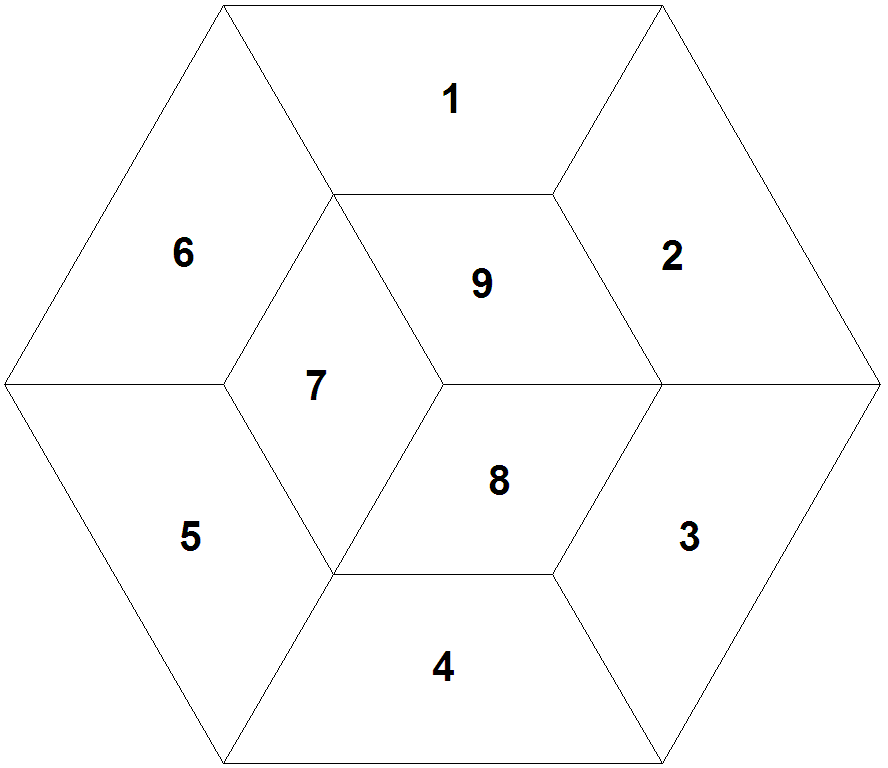
\includegraphics[width=0.55\linewidth]{figures/cyccore_1.png}
\caption{Standard cyclic core (Coppola 2007, Fig.~1): outer cells $1$--$6$
are collapsible; inner $7$--$9$ are not.}
\label{fig:cyccore}
\end{figure}

\section{Counterexample sharpness on Layer-0 cores}
\label{sec:negative}

\begin{itemize}
\item \textbf{Swap-only and force-include.}  Proposition~\ref{prop:layer0-cex}:
$9\times 9$ swap counterexample and $12\times 13$ bridged double-$6$-cycle
include counterexample (Lean \texttt{native\_decide}).
\item \textbf{Single-face covering collapse.}  Vacuous on the 2007 core (C21);
Horn retraction is non-vacuous on the same instance.
\item \textbf{Shotgun shelling.}  Simultaneous admissible free-face batches are
\emph{not} optimality-preserving (C9; Table~\ref{tab:shotgun}).
\item \textbf{Classical collapse-branch.}  On $n=5$ samples the implemented
admissibility-guarded branch disagrees with exact optima; certified synthesis
uses plain B\&B / Espresso-Horn windows, with collapse-branch as a comparator.
\end{itemize}
Visual $2$D intuition for the older grid far-side story is in
\texttt{intuition\_examples.pdf}.

\begin{table}[h]
\centering\small
\caption{Audit of the collapse-branch and of shotgun (simultaneous) collapse against an exact oracle on Boolean covering instances. Sequential: instances where the collapse branch fired / disagreements with the exact optimum. Shotgun rules: nontrivial instances (a batch was applied) / cost mismatches / reduced tables left infeasible. ``none'': all admissible pairs; ``rows'': pairwise row-disjoint faces; ``safe'': row-disjoint plus a coverability guard.}
\label{tab:shotgun}
\resizebox{\linewidth}{!}{\begin{tabular}{lrrrr}
\hline
set & sequential & shotgun none & shotgun rows & shotgun safe \\
\hline
n=3 (all) & 0 / 0 & 0 / 0 / 0 & 0 / 0 / 0 & 0 / 0 / 0 \\
n=4 (all) & 330 / 0 & 864 / 672 / 672 & 864 / 672 / 672 & 864 / 33 / 0 \\
n=5 (sample 1500) & 36 / 2 & 72 / 40 / 37 & 72 / 40 / 37 & 72 / 16 / 0 \\
\hline
\end{tabular}}
\end{table}


\section{Conclusion}

The cyclic core is a cubical complex: Roth extremals (essentials and free faces),
Horn retraction, Espresso-family heuristics, and LP/TU bounds jointly explain
when covering is easy, approximable, or hard---and how to escape
\texttt{sccc}-locked local minima with certified windows.

\paragraph{Status of the formalization.}  The Lean~4 library builds from a bare
\texttt{lake build} with no unfinished proofs.  It contains Layer-0 legal
expansion / zero-loss / blob lemmas (\textsf{Layer0CubeArray.lean}); Horn
retraction, cylinder, complement duality, and chain-window lemmas
(\textsf{HornChains.lean}); Roth extremal hierarchy, \texttt{sccc}-stall escape,
and tightened LP/MIS window (\textsf{RothEspressoHorn.lean}); plus older
\textsf{StarLink}/\textsf{LocalTransform}/\textsf{OutComplex} companions for the
intuition note.  It does \emph{not} contain a general TU theorem.

\paragraph{Program companion.}  Paper~E~\cite{paperE} measures Horn covering on
medical voxels / 2007 cores, spine windows, and classic Espresso / ABC-Horn SOP
(claims C56--C58).

\paragraph{Future work.}  Larger $.pla$ suites; Bala-led TU/neutralization of
cyclic-core residues; Lusternik--Schnirelmann cup-length lower bounds (Python
tested only).

\section*{Acknowledgments}
The author thanks Richard Weiss for early discussions and collaboration on
the 2006--2007 manuscript \emph{Cyclic Core Covering and Finite Cell Complexes}
\cite{coppola2006sat,coppola2007}, from which this work grew.

\bibliographystyle{plain}
\begin{thebibliography}{99}

\bibitem{paperE}
A.~J. Coppola.
\newblock Horn retraction and controlled chains for certified TDA spines, with
Espresso/ABC extensions.
\newblock TopoSpine Paper~E (arXiv Wave~1 companion; ID pending), 2026.

\bibitem{quine1952}
W.~V. Quine.
\newblock The problem of simplifying truth functions.
\newblock \emph{Amer. Math. Monthly}, 59(8):521--531, 1952.

\bibitem{mccluskey1956}
E.~J. McCluskey.
\newblock Minimization of Boolean functions.
\newblock \emph{Bell System Tech.\ J.}, 35(6):1417--1444, 1956.

\bibitem{brayton1984}
R.~K. Brayton, G.~D. Hachtel, C.~T. McMullen, and A.~L. Sangiovanni-Vincentelli.
\newblock \emph{Logic Minimization Algorithms for VLSI Synthesis}.
\newblock Kluwer, 1984.

\bibitem{mcgeer1993}
P.~C. McGeer, J.~V. Sanghavi, R.~K. Brayton, and A.~L. Sangiovanni-Vincentelli.
\newblock Espresso-Signature: a new exact minimizer for logic functions.
\newblock \emph{IEEE Trans.\ VLSI}, 1(4):432--440, 1993.

\bibitem{fiser2003}
P.~Fi\v{s}er and J.~Hlavi\v{c}ka.
\newblock BOOM---a heuristic Boolean minimizer.
\newblock \emph{ICCAD}, 2003.

\bibitem{coudert1994}
O.~Coudert.
\newblock Two-level logic minimization: an overview.
\newblock \emph{Integration}, 17(2):97--140, 1994.

\bibitem{goldberg2000}
E.~I. Goldberg, L.~P. Carloni, T.~Villa, R.~K. Brayton, and A.~L. Sangiovanni-Vincentelli.
\newblock Negative thinking in branch-and-bound: the case of unate covering.
\newblock \emph{IEEE TCAD}, 19(3):281--294, 2000.

\bibitem{roth1957}
J.~P. Roth.
\newblock Algebraic topological methods for the synthesis of switching systems I.
\newblock \emph{Trans. Amer. Math. Soc.}, 88(2):301--326, 1957.

\bibitem{coppola1989}
A.~J. Coppola.
\newblock New methods in the analysis of logic minimization data and algorithms.
\newblock \emph{DAC}, 1989.

\bibitem{coppola2007}
A.~J. Coppola and R.~Weiss.
\newblock Cyclic core covering and finite cell complexes.
\newblock Technical report, Evergreen State College, 2007.

\bibitem{coppola2006sat}
A.~J. Coppola and R.~Weiss.
\newblock Cyclic core covering and finite cubical cell complexes.
\newblock SAT 2006 submission.

\bibitem{dey2011}
T.~K. Dey, A.~N. Hirani, and B.~Krishnamoorthy.
\newblock Optimal homologous cycles, total unimodularity, and linear programming.
\newblock \emph{SIAM J. Comput.}, 40(4):1026--1040, 2011.

\bibitem{ks2018}
B.~Krishnamoorthy and G.~Smith.
\newblock Non total-unimodularity neutralized simplicial complexes.
\newblock \emph{Discrete Appl. Math.}, 240:44--62, 2018.

\bibitem{goresky2024}
M.~Goresky.
\newblock Topological aspects of Boolean functions.
\newblock \emph{PAMQ}, 20(3), 2024.

\bibitem{psrt2025}
Persistent Stanley--Reisner theory.
\newblock \emph{Foundations of Data Science}, 2025.

\bibitem{bjorner2003}
A.~Bj\"orner.
\newblock Nerves, fibers and homotopy groups.
\newblock \emph{J. Combin. Theory Ser. A}, 102(1):88--93, 2003.

\bibitem{francisco2013}
C.~A. Francisco, J.~Mermin, and J.~Schweig.
\newblock A survey of Stanley--Reisner theory.
\newblock 2013.

\bibitem{cohen1973}
M.~M. Cohen.
\newblock \emph{A Course in Simple-Homotopy Theory}.
\newblock Springer, 1973.

\end{thebibliography}

\end{document}
